% Author : Prakash
% Date   : 2022-11-23 16:44
% vim: ai ts=4 sts=4 et sw=4 ft=tex

\documentclass[a4paper,12pt]{article}
\usepackage[margin=38mm]{geometry}

\usepackage{amsmath}
\usepackage{amssymb}
\usepackage{graphicx}
\usepackage{parskip}
\usepackage{tikz}
\usepackage{minted}
\usepackage{hyperref}
\usepackage{pgfplots}
\usepackage{tikz}
\usepackage{multicol}

\usetikzlibrary{patterns,plotmarks}


\title{Simulation of helicoil material.}
\author{Prakash Gautam}

\graphicspath{{../../asset}}

\input{pgf-preamble.tex}


\begin{document}
    \maketitle
    %The macro used in the primary simulation.
    %\inputminted{ini}{../../asset/files/primary-sim-macro.mac}
\section{Primary simulation}
    A total of 1000 jobs were submitted of which 988 were completed. This make as a total of 98,800,000 primary events simulated.  The distribution of events that hit the new geometry is shown in Figure \ref{fig:primary-hit-det}. The total events that hit helicoil material (across all simulated files) is: 2091094 (area under the curve in \ref{fig:primary-hit-det}).

    
    \begin{figure}[h!]
        \centering
        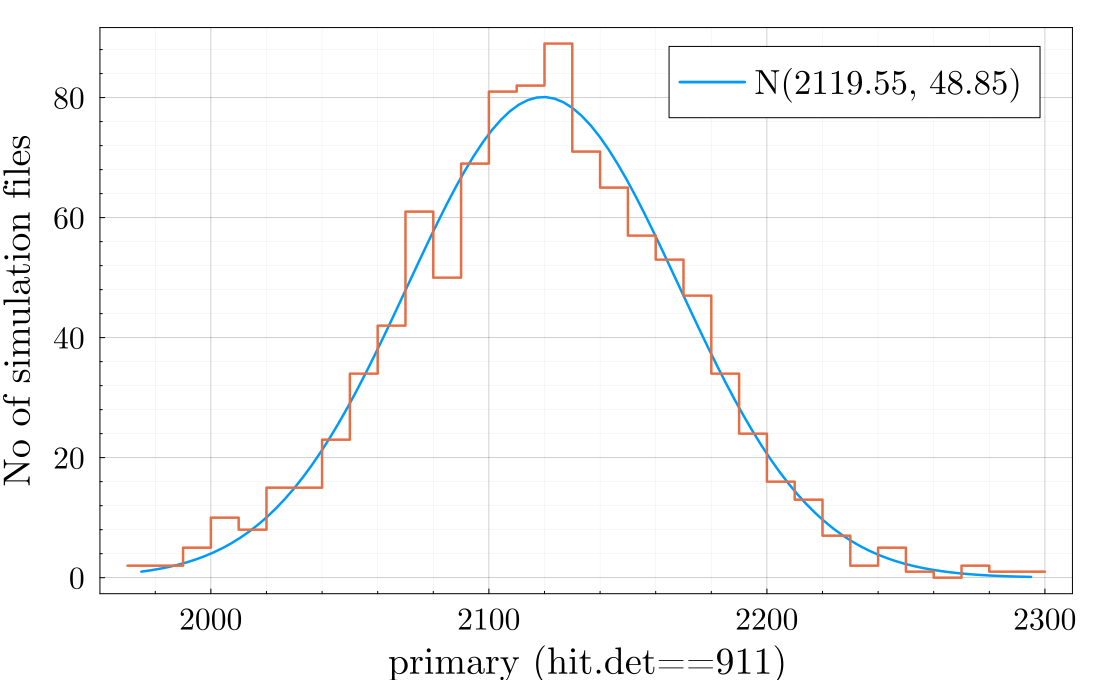
\includegraphics[width=1\linewidth]{image/helicoil-20221121-113016-img-primary-det-hit-count-hist-not-normalized.png}
        \caption{The distribution number of hits helicoil material (hit.det==911). The total primary simulated in each files is 100,000. So only about $0.2$\% make it to the helicoil material. The continuous curve is a gaussian fitted oveer histogram.}
        \label{fig:primary-hit-det}
    \end{figure}


    These hits can be various different particles. The particle of interest for the secondary is the primary electrons (hit.trid==1).  The distribution of number of hit of these electrons per fileis showin in \ref{fig:primary-dist}. The total electron events hitting the helicoil materials is 10395. This ratio is
    \begin{align*}
        \frac{10395}{98800000} = 1.05 \times 10^{-4}
    \end{align*}



    \begin{figure}[h!]
        \centering
        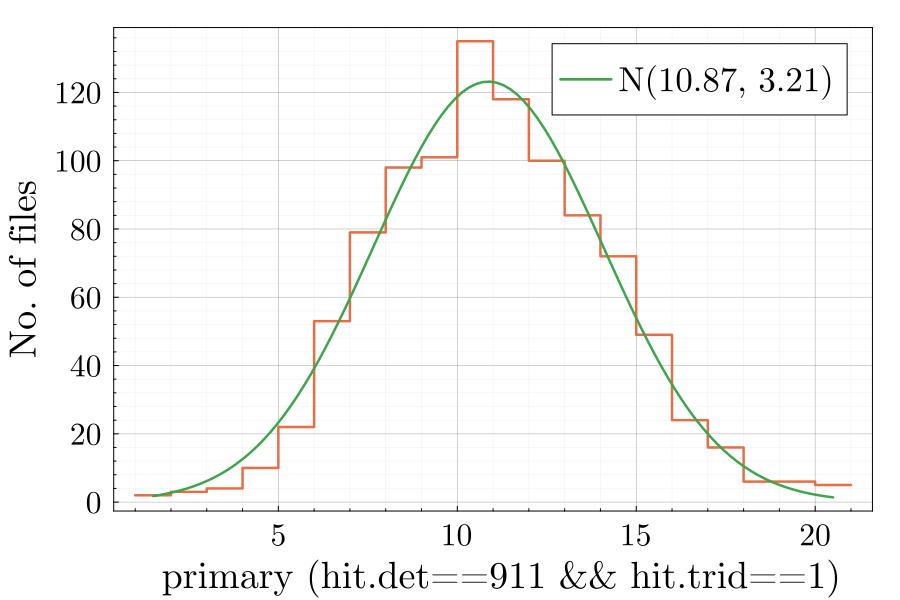
\includegraphics[width=1\linewidth]{image/helicoil-20221121-113016-img-primary-trid-hit-count-hist.png} \caption{The distribution of No. of primary electrons (hit.trid==1) that hit the new geometry (hit.det ==911).}
        \label{fig:primary-dist}
    \end{figure}

    All of these simulated files is combined into a single primary ``Skimmed" root tree containing only the hit branch with "hit.trid==1 \&\& hit.det==911" (here 911 corresponds to the detector id for the helicoil geometry).

\section{Secondary simulation}
    With this skimmed file as an input generator to the simulation, a total 100 secondary simulation is run with 100,000 events each. One of the job failed with 9,900,000 secondary events.
    \begin{figure}[h!]
        \centering
        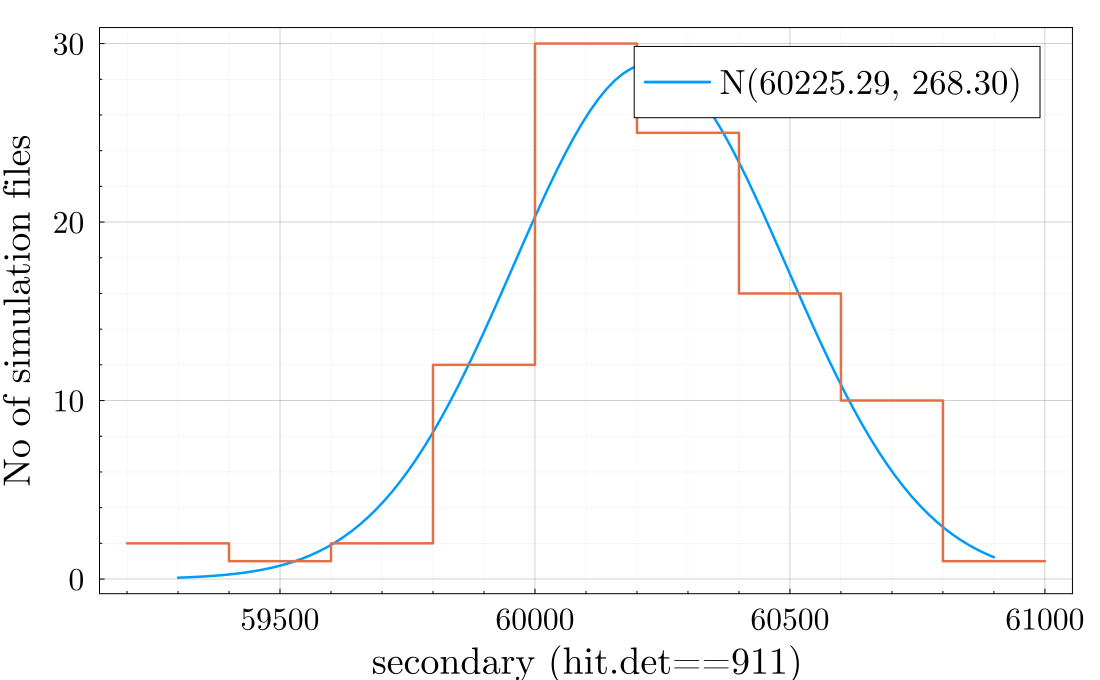
\includegraphics[width=1\linewidth]{image/helicoil-20221121-113016-img-secondary-det-hit-count-hist-not-normalized.png}
        %\input{../../asset/image/helicoil-20221121-113016-img-113016-secondary-det-hit-count-hist-not-normalized.tex}
        \caption{The distribution of hit in the helicoil geometry for secondary simulation. Only $\sim 60$\% of the events hit the new geometry.}
        \label{fig:sec-hit-det-distrib}
    \end{figure}

    The distribution of hits in the secondary simulation files is shown in Figure \ref{fig:sec-hit-det-distrib}. 

    \begin{figure}[h!]
        \centering
        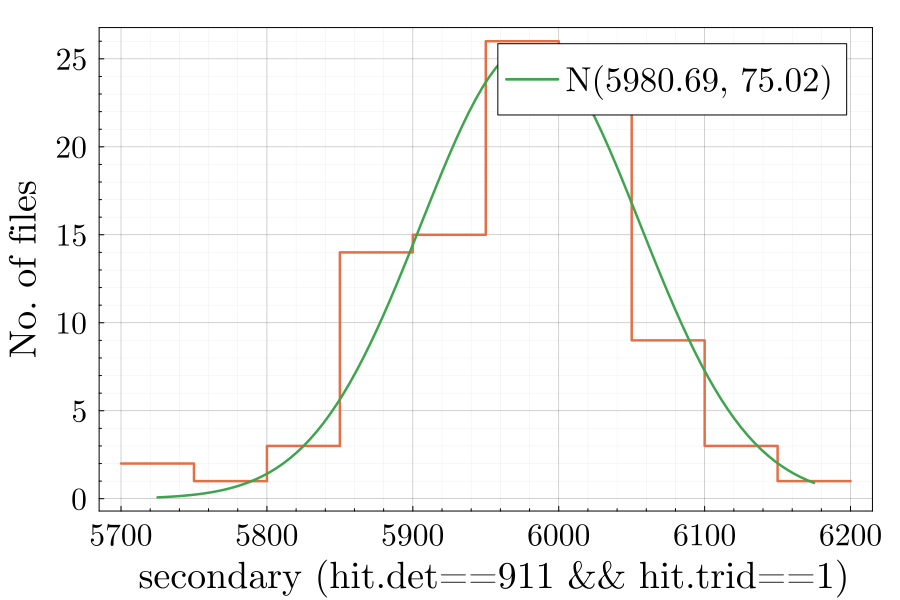
\includegraphics[width=1\linewidth]{image/helicoil-20221121-113016-img-secondary-trid-hit-count-hist.png}
        \caption{The distribution of No. of electrons (hit.trid==1) that hit the new geometry (hit.det ==911)}
        \label{fig:sec-hit-911-trid-1}
    \end{figure}

    For the final detector the event distribution is shown in Figure \ref{fig:sec-hit-28-no-trid}.
    \begin{figure}[h!]
        \centering
        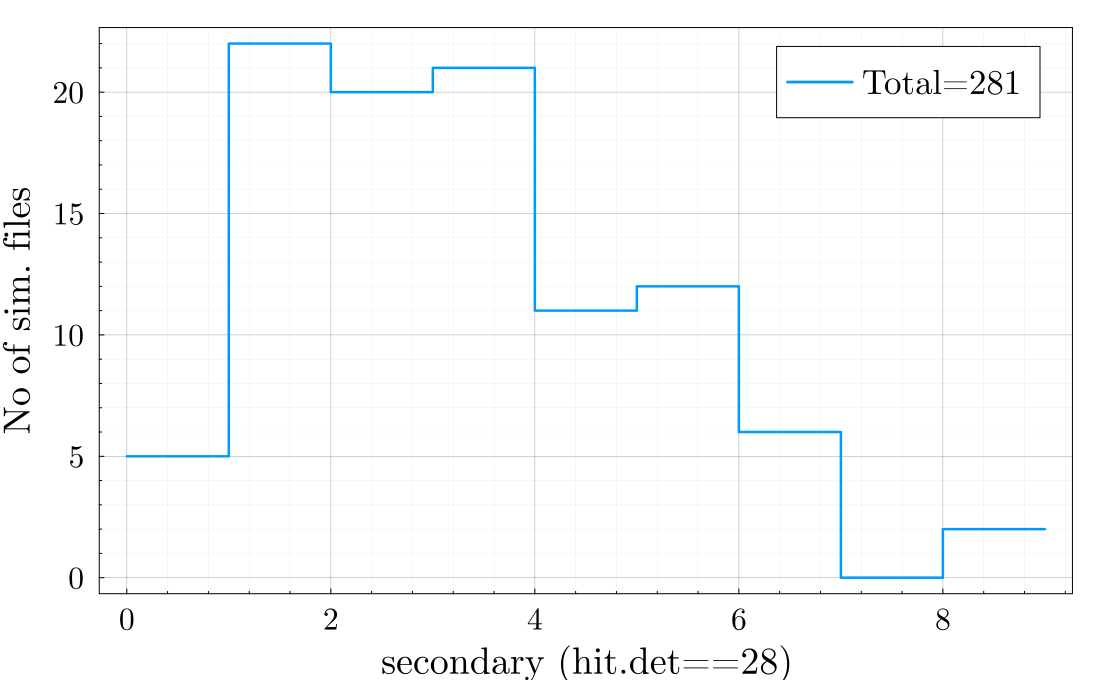
\includegraphics[width=0.9\linewidth]{image/helicoil-20221121-113016-secondary-fin-det-hit.png}
        \caption{The distribution of number of events per 100,000 secondary simulation in the final detetector (hit.det==28). A total of 281 events make it to the detector, of the total simulated 9,900,000 secondary events.}
        \label{fig:sec-hit-28-no-trid}
    \end{figure}
    \begin{align*}
        \frac{281}{9900000} = 2.83 \times 10^{-5}
    \end{align*}
    \subsection{Energy distribution}
    All of the secondary simulation files are combined into a single root file.
    \begin{table}[h!]
        \centering
        \begin{tabular}{r|r|rrr}
            &  Primary($9.88 \times 10^{7}$)  &  \multicolumn{3}{c}{Secondary($9.9 \times 10^{6}$)} \\
            \hline
            Energy[hit.e] (MeV) & det==911\&\& trid==1  & det == 911 & det==911\&\& trid==1  &  det == 28 \\
            \hline
            \hline
            0.00 - 0.01         &    0 &      36 &       0 &       0 \\
            0.01 - 0.10         &    0 &  191606 &       0 &     182 \\
            0.10 - 1.00         &   11 & 3876080 &   72764 &      85 \\
            1.00 - 10.00        &  829 &  889937 &  459323 &      10 \\
            10.00 - 100.00      & 9018 &   66011 &   58572 &       2 \\
            100.00 - 1000.00    &  432 &    6026 &      34 &       2 \\
            1000.00 - 100000.00 &  104 &      61 &       0 &       0 \\
            \hline
            Total               & 10394 & 5029757 & 5029757 &     281\\
             \hline
        \end{tabular} ~
    \end{table}
    \begin{table}[h!]
        \centering
        \begin{tabular}{r|r|rr}
            &  Primary($9.88 \times 10^{7}$)  &  \multicolumn{2}{c}{Secondary($9.9 \times 10^{6}$)} \\
            \hline
            Energy[hit.e] (MeV) & det==911\&\& trid==1  & det == 911 \&\& trid==1 & det == 28 \\
            \hline
            \hline
            0.00 - 0.01         &    0 &     0 \\
            0.01 - 0.10         &    0 &   182 \\
            0.10 - 1.00         &   11 &    85 \\
            1.00 - 10.00        &  829 &    10 \\
            10.00 - 100.00      & 9018 &     2 \\
            100.00 - 1000.00    &  432 &     2 \\
            1000.00 - 100000.00 &  104 &     0 \\
             \hline
             Total                & 10394     & 281 
        \end{tabular} ~
    \end{table}
    \bibliographystyle{ieeetr85}
    \bibliography{Neutrino.bib}
\end{document}

